\documentclass[11pt]{article}
\usepackage{amsmath,amssymb,amsmath,amsthm,amsfonts}
\usepackage{latexsym,graphicx}
\usepackage{fullpage,color}
\usepackage{url,hyperref}
\usepackage{natbib}
\usepackage{graphicx,subfigure}
\usepackage{algorithm}
\usepackage{algorithmic}
\usepackage{listings}
\usepackage{xcolor}
\usepackage{color}

\numberwithin{equation}{section}

\pagestyle{plain}

\setlength{\oddsidemargin}{0in}
\setlength{\topmargin}{0in}
\setlength{\textwidth}{6.5in}
\setlength{\textheight}{8.5in}

\newtheorem{fact}{Fact}[section]
\newtheorem{question}{Question}[section]
\newtheorem{lemma}{Lemma}[section]
\newtheorem{theorem}[lemma]{Theorem}
\newtheorem{assumption}[lemma]{Assumption}
\newtheorem{corollary}[lemma]{Corollary}
\newtheorem{prop}[lemma]{Proposition}
\newtheorem{claim}{Claim}[section]
\newtheorem{remark}{Remark}[section]
\newtheorem{definition}{Definition}[section]
\newtheorem{prob}{Problem}[section]
\newtheorem{conjecture}{Conjecture}[section]
\newtheorem{property}{Property}[section]


\def\alp{\mbox{\boldmath$\alpha$\unboldmath}}
\def\bet{\mbox{\boldmath$\beta$\unboldmath}}
\def\epsi{\mbox{\boldmath$\epsilon$\unboldmath}}
\def\etab{\mbox{\boldmath$\eta$\unboldmath}}
\def\ph{\mbox{\boldmath$\phi$\unboldmath}}
\def\pii{\mbox{\boldmath$\pi$\unboldmath}}
\def\Ph{\mbox{\boldmath$\Phi$\unboldmath}}
\def\Ps{\mbox{\boldmath$\Psi$\unboldmath}}
\def\ps{\mbox{\boldmath$\psi$\unboldmath}}
\def\tha{\mbox{\boldmath$\theta$\unboldmath}}
\def\Tha{\mbox{\boldmath$\Theta$\unboldmath}}
\def\muu{\mbox{\boldmath$\mu$\unboldmath}}
\def\Si{\mbox{\boldmath$\Sigma$\unboldmath}}
\def\si{\mbox{\boldmath$\sigma$\unboldmath}}
\def\Gam{\mbox{\boldmath$\Gamma$\unboldmath}}
\def\Lam{\mbox{\boldmath$\Lambda$\unboldmath}}
\def\De{\mbox{\boldmath$\Delta$\unboldmath}}
\def\Ome{\mbox{\boldmath$\Omega$\unboldmath}}
\def\Pii{\mbox{\boldmath$\Pi$\unboldmath}}
\def\varepsi{\mbox{\boldmath$\varepsilon$\unboldmath}}

\def\argmax{\mathop{\rm argmax}}
\def\argmin{\mathop{\rm argmin}}
\def\bias{\mathsf{bias}}
\def\var{\mathsf{var}}
\def\sgn{\mathsf{sgn}}
\def\tr{\mathsf{tr}}
\def\rk{\mathrm{rank}}
\def\poly{\mathrm{poly}}
\def\diag{\mathsf{diag}}
\def\st{\mathsf{s.t.}}

\newcommand{\red}[1]{{\color{red}#1}}



\lstset{ %
extendedchars=false,            % Shutdown no-ASCII compatible
language=R,                % choose the language of the code
xleftmargin=1em,
xrightmargin=1em,
basicstyle=\footnotesize,    % the size of the fonts that are used for the code
tabsize=3,                            % sets default tabsize to 3 spaces
numbers=left,                   % where to put the line-numbers
numberstyle=\tiny,              % the size of the fonts that are used for the line-numbers
stepnumber=1,                   % the step between two line-numbers. If it's 1 each line
                                % will be numbered
numbersep=5pt,                  % how far the line-numbers are from the code   %
backgroundcolor=\color{white}, % choose the background color. You must add \usepackage{color}
showspaces=false,               % show spaces adding particular underscores
showstringspaces=false,         % underline spaces within strings
showtabs=false,                 % show tabs within strings adding particular underscores
frame=single,                 % adds a frame around the code
%captionpos=b,                   % sets the caption-position to bottom
breaklines=true,                % sets automatic line breaking
breakatwhitespace=false,        % sets if automatic breaks should only happen at whitespace
%title=\lstname,                 % show the filename of files included with \lstinputlisting;
%                                % also try caption instead of title
mathescape=true,escapechar=?    % escape to latex with ?..?
escapeinside={\%*}{*)},         % if you want to add a comment within your code
%columns=fixed,                  % nice spacing
%morestring=[m]',                % strings
%morekeywords={%,...},%          % if you want to add more keywords to the set
%    break,case,catch,continue,elseif,else,end,for,function,global,%
%    if,otherwise,persistent,return,switch,try,while,...},%
}


\begin{document}


\title{FE-511-B: Final Project}

\author{Sean Trinh}

%\date{ }

\maketitle


\section{Problem Description}

\paragraph{Introduction.}

The state of modern economies is measured in gross domestic product (GDP), or the total value of final goods produced and services provided in a country during one year. In other words, GDP is an aggregate calculation of a country's consumer spending, business investment, government spending, and net exports in a given time period. An important distinction to note is that nominal GDP is evaluated at current market prices, which means that its value is affected by inflation or deflation. Read GDP, on the other hand, is not.

In the United States, there are two major stock indexes: the S\&P 500 and the Dow Jones Industrial Average (DJIA). The S\&P 500 is an index that includes 500 companies, spanning all sorts of industries, and is based on each individual company's market capitalization, meaning companies with higher market capitalization will have a bigger impact on the calculation of the index than companies with lower market capitalization. The DJIA on the other hand includes thirty companies, spanning some of the major industries, and is based on each individual company's stock price.

Economists and investors alike are interested in finding ways to better track and predict the state of the US economy. For example, economists have done a lot of research into the yield curves of the US fixed income market. Since the 1970s, very time the yield curves in the United States have inverted, meaning yields on short term bonds have risen above the yields on long term bonds, the US has entered a recession shortly after.

This project will seek to explore the validity of using either the S\&P 500 or the DJIA or both in tracking the state, health, and growth of the US economy. As the S\&P 500 and DJIA have much more frequent and regular reportings than US GDP, which is reported on a quarterly basis, it may be beneficial to economists and investors to keep track of the more frequent reportings of both indexes in order to predict whether they should be optimistic, or bullish, on the economy or pessimistic, or bearish, on the economy. In other words, does positive growth in the S\&P 500 and/or DJIA indexes necessarily predict a positive growth in US GDP, and vice-versa? If there exists a positive correlation between the indexes and US GDP, do the indexes overstate or understate how well the economy is doing?

\paragraph{Thesis.}
The S\&P 500 and DJIA keep track of what each index deems as the top 500 and top 30 companies in the United States, respectively. Because of this, each index may be prone to overstating how well the overall US economy is doing, because neither is keeping track of smaller companies that may be performing poorly compared to the tracked, top companies. However, since these companies in theory make up a large and significant portion of the economy, it should still be the case that positive growth in these indexes should predict positive growth in US GDP.

Because of this, positive growth in the S\&P 500 and DJIA indexes predict a positive growth is US GDP, and vice-versa, but are prone to overstating how well the economy is doing.

\section{Data and Methodology}

\paragraph{Data.} 
The data that will be used to conduct the regressions and analyses includes quarterly data on the nominal US GDP, quarterly S\&P 500 data, and quarterly DJIA data. Although S\&P 500 and DJIA data is reported more frequently than quarterly, quarterly data must be used in order to do proper regressions on nominal US GDP, which is only reported quarterly. Also, since the data for nominal US GDP only goes back to the 1940s, all sets of data will be scoped to start at the earliest quarterly reporting of nominal US GDP data and end at the most recent quarterly reporting.

\paragraph{Methodology.}
Three regressions to test the hypothesis will be done, all of which will be done using the programming language, R. First, a linear regression will be done to determine the relationship between the S\&P 500 and US Nominal GDP. Standard regression results will be reported and analyzed, and a regression equation like the following will be produced:

\[ US Nominal GDP_{t} = \alp*S\&P500_{t} + \epsi \]

A second linear regression will be done to determine the relationship between the DJIA and US Nominal GDP. Standard regression results will be reported and analyzed, and a regression equation like the following will be produced:

\[ US Nominal GDP_{t} = \alp*DJIA_{t} + \epsi \]

Finally, a multivariate linear regression will be done to determine the relationship between the S\&P 500 and DJIA and US Nominal GDP. Standard regression results will be reported and analyzed, and a regression equation like the following will be produced:

\[ US Nominal GDP_{t} = \alp*S\&P500_{t} + \bet*DJIA_{t} + \epsi \]

Using the regression results and equations produced from these three regressions, an analysis will be conducted, and a conclusion on the hypothesis will be made.

Common studies on indicators of GDP growth will lag US GDP in response to a variable. In other words, regressions sometimes try to see how a change in variable affects GDP a number of quarters later. An example regression would look like the following:

\[ US Nominal GDP_{t+n} = \alp*S\&P500_{t} + \bet*DJIA_{t} + \epsi \]

In the above equations, t represents the variables at a given time. In only the above equation does n represent a number of quarters after the given time, hencing lagging. Lagging will not be done with these regressions, because the idea of this study and hypothesis is to see if either or both of the indexes are able to simulatenously track the direction of GDP so that economists and investors can estimate or predict the quarter's GDP before it is reported. In other words, the idea of this study is not to see how changes in either index affect GDP in future quarters. In theory, GDP is strongly correlated to both indexes and mostly made up of the value produced by and performances of companies in those indexes in a specific, given quarter, not future or previous quarters.

\section{Regression, Code, and Results}

\paragraph{S\&P 500 and US Nominal GDP}

\subparagraph{Code.}
The following R code was used to load the quarterly data for the S\&P 500 and US Nominal GDP and run a linear regression on the data to produce a regression equation and summary. The correlation coefficient between the two variables was also produced.

\vspace{3mm}
\begin{lstlisting}[language=R]
library("readxl")
my_data <- as.data.frame(read_excel("Documents/Classes/FE/fe511/fe_511_final_project/fe_511_data.xlsx"))
us_nominal_gdp <- my_data[,"us_nominal_gdp"]
sp_500 <- my_data[,"sp_500"]
regression_sp_500 <- lm(us_nominal_gdp ~ sp_500)
summary(regression_sp_500) #Summary of the regression
cor(us_nominal_gdp, sp_500) #Correlation coefficient between the two variables

\end{lstlisting}
\vspace{3mm}

\subparagraph{Regression.}
Figure~\ref{fig:model1} outlines the results of the linear regression on US Nominal GDP and the S\&P 500. Additionally, the correlation coefficient between the two variables was reported to be \textbf{0.9582932}.

The regression equation, based on the results, is as follows:

\[ US Nominal GDP_{t} = 8.3843*S\&P500_{t} + 1340.9416 \]

%---------------------------------Figure---------------------------------%
\begin{figure}
	\begin{center}
		{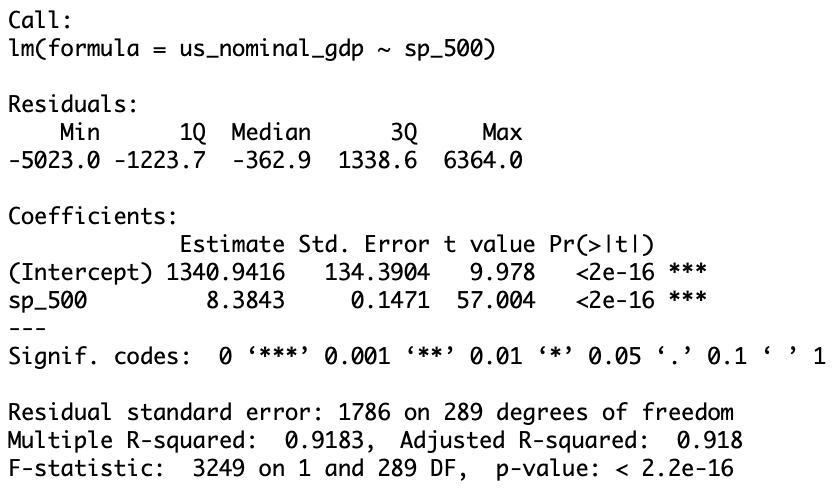
\includegraphics[width=0.75\textwidth]{regression_results_sp500.png}}
	\end{center}
	\caption{Regression Results - S\&P 500.}
	\label{fig:model1}
\end{figure}
%---------------------------------Figure---------------------------------%

\paragraph{DJIA and US Nominal GDP}

\subparagraph{Code.}
The following R code was used to load the quarterly data for the DJIA and US Nominal GDP and run a linear regression on the data to produce a regression equation and summary. The correlation coefficient between the two variables was also produced.

\vspace{3mm}
\begin{lstlisting}[language=R]
library("readxl")
my_data <- as.data.frame(read_excel("Documents/Classes/FE/fe511/fe_511_final_project/fe_511_data.xlsx"))
us_nominal_gdp <- my_data[,"us_nominal_gdp"]
djia <- my_data[,"djia"]
regression_djia <- lm(us_nominal_gdp ~ djia)
summary(regression_djia) #Summary of the regression
cor(us_nominal_gdp, djia) #Correlation coefficient between the two variables
\end{lstlisting}
\vspace{3mm}

\subparagraph{Regression.}
Figure~\ref{fig:model2} outlines the results of the linear regression on US Nominal GDP and the DJIA. Additionally, the correlation coefficient between the two variables was reported to be \textbf{0.9603199}.

The regression equation, based on the results, is as follows:

\[ US Nominal GDP_{t} = 0.9468*DJIA_{t} + 1397 \]

%---------------------------------Figure---------------------------------%
\begin{figure}
	\begin{center}
		{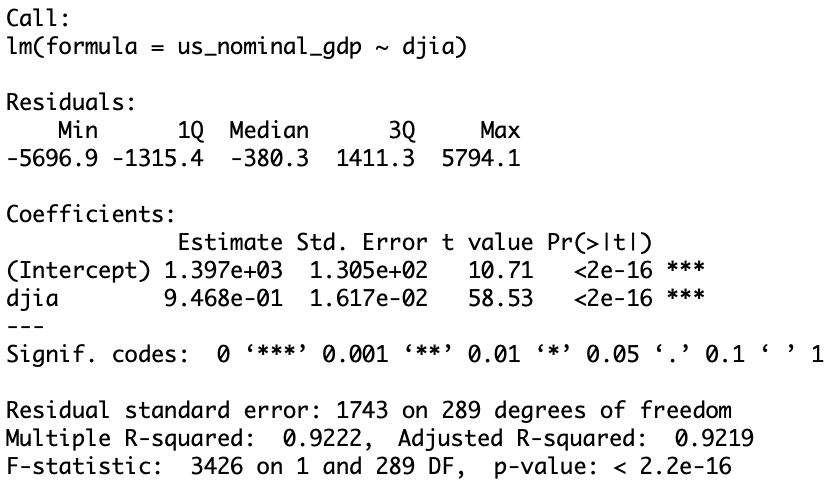
\includegraphics[width=0.75\textwidth]{regression_results_djia.png}}
	\end{center}
	\caption{Regression Results - DJIA.}
	\label{fig:model2}
\end{figure}
%---------------------------------Figure---------------------------------%

\paragraph{DJIA, S\&P 500, and US Nominal GDP}

\subparagraph{Code.}
The following R code was used to load the quarterly data for the S\&P 500, DJIA, and US Nominal GDP and run a multivariate linear regression on the data to produce a regression equation and summary.

\vspace{3mm}
\begin{lstlisting}[language=R]
library("readxl")
my_data <- as.data.frame(read_excel("Documents/Classes/FE/fe511/fe_511_final_project/fe_511_data.xlsx"))
us_nominal_gdp <- my_data[,"us_nominal_gdp"]
sp_500 <- my_data[,"sp_500"]
djia <- my_data[,"djia"]
regression_both <- lm(us_nominal_gdp ~ sp_500 + djia)
summary(regression_both) #Summary of the regression
\end{lstlisting}
\vspace{3mm}

\subparagraph{Multivariate Regression.}
Figure~\ref{fig:model3} outlines the results of the linear regression on US Nominal GDP and the S\&P 500 and DJIA.

The regression equation, based on the results, is as follows:

\[ US Nominal GDP_{t+n} = 0.6461*S\&P500_{t} + 0.8742*DJIA_{t} + 1390.5869 \]

%---------------------------------Figure---------------------------------%
\begin{figure}
	\begin{center}
		{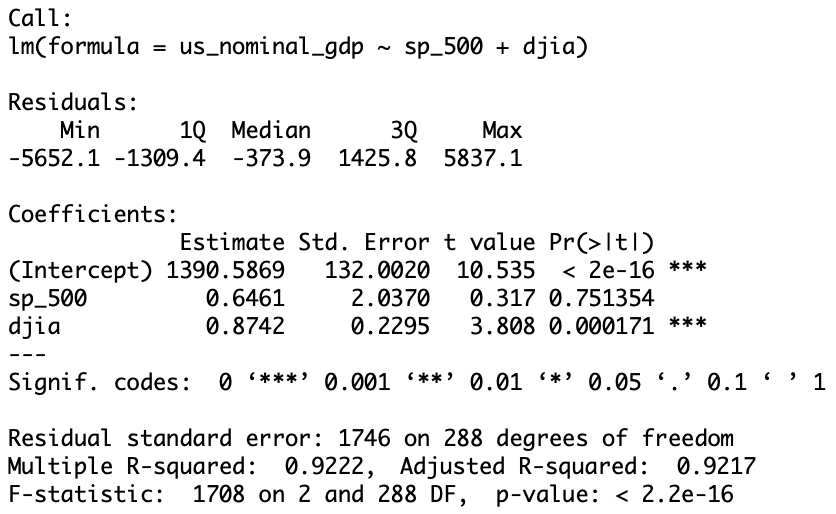
\includegraphics[width=0.75\textwidth]{regression_results_both.png}}
	\end{center}
	\caption{Multivariate Regression Results - S\&P 500 and DJIA.}
	\label{fig:model3}
\end{figure}
%---------------------------------Figure---------------------------------%

\section{Discussion}

\paragraph{Observations.}
Test. Test. Put some observations here.

\paragraph{Conclusion.}
Test. Test. Either reject the hypothesis or fail to reject the hypothesis here.

\paragraph{Further Steps.}
Test. Test. Put down some thoughts as to what can be done next to further test the hypothesis/main idea.


%\newpage
\bibliographystyle{plain}
\bibliography{reference}


\end{document}
